\section{Chức năng tìm kiếm}
\subsection{Tìm kiếm theo từ khóa}
Chức năng cho phép người dùng nhập từ khóa (tên bài hát, ca sĩ, thể loại, v.v.) vào thanh tìm kiếm để nhận kết quả gợi ý phù hợp. Kết quả sẽ hiển thị danh sách các bài hát, ca sĩ, album tương ứng và cho phép lọc.
\begin{figure}[H]
    \centering
    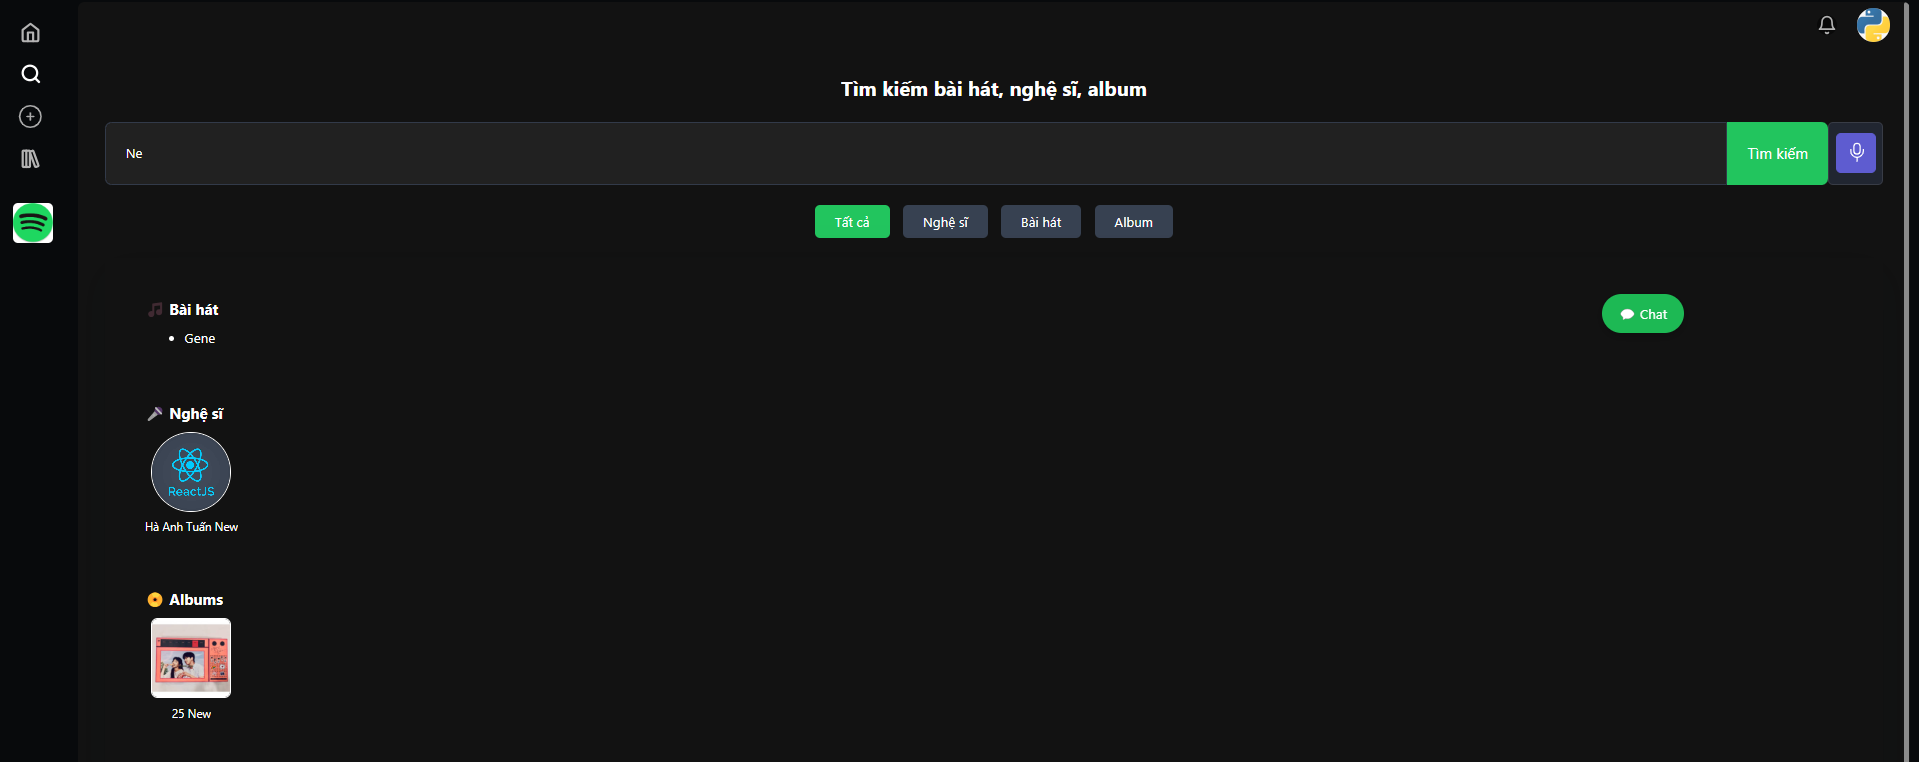
\includegraphics[width=1\textwidth]{imgs/chap5/tim_kiem_1.png}
    \caption{Giao diện tìm kiếm theo từ khóa}
\end{figure}

\begin{figure}[H]
    \centering
    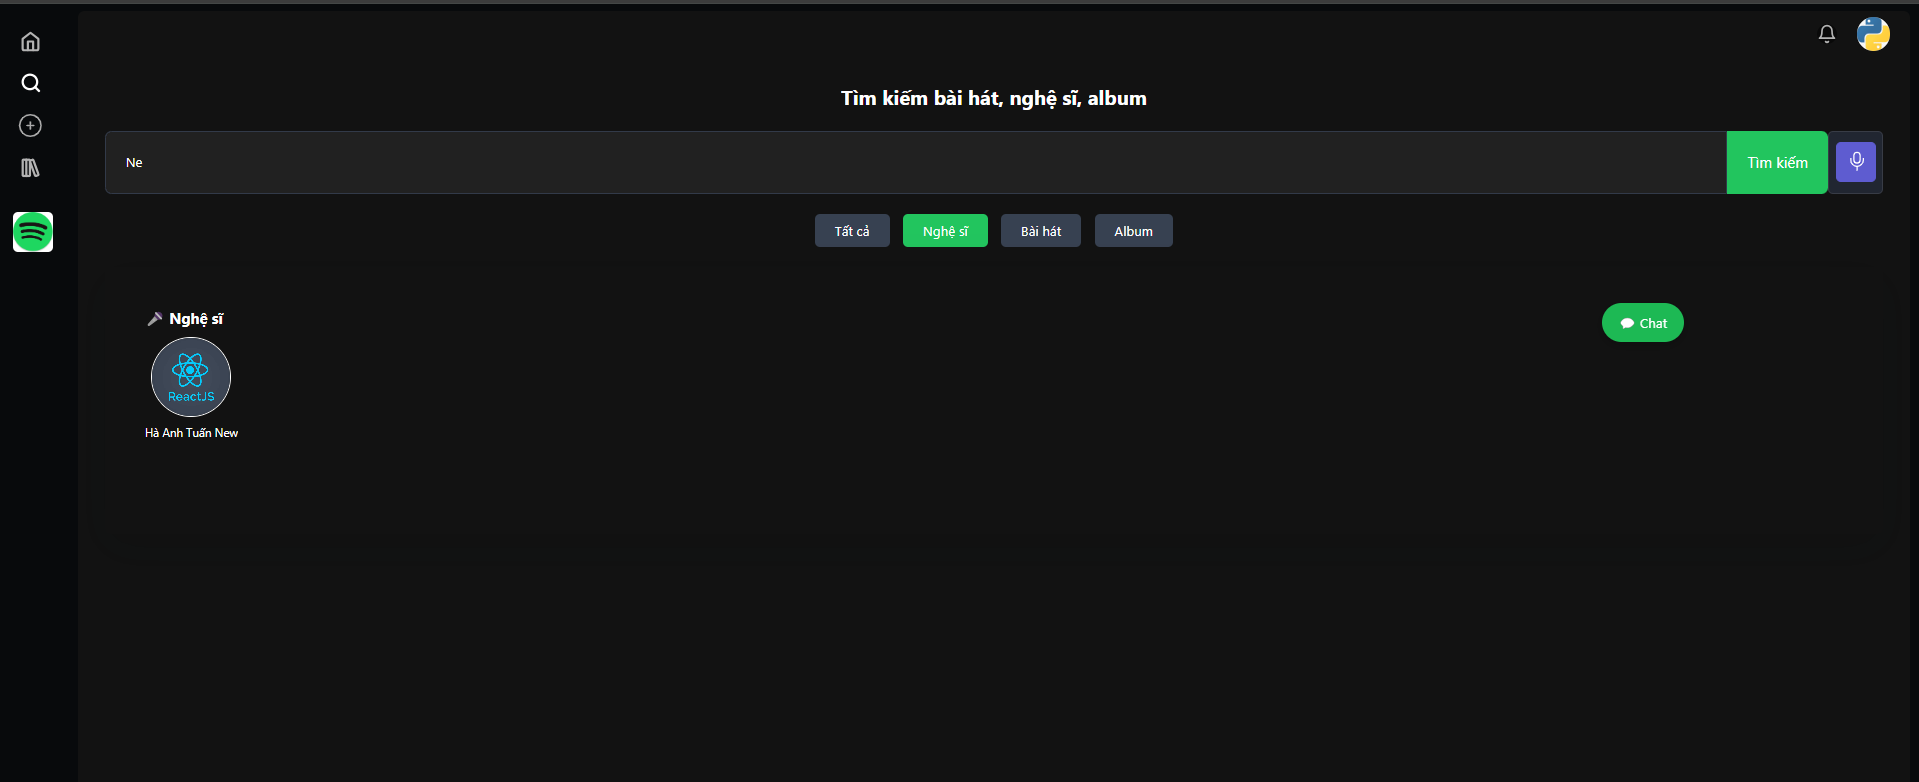
\includegraphics[width=1\textwidth]{imgs/chap5/tim_kiem_2.png}
    \caption{Giao diện tìm kiếm nghệ sĩ}
\end{figure}

\begin{figure}[H]
    \centering
    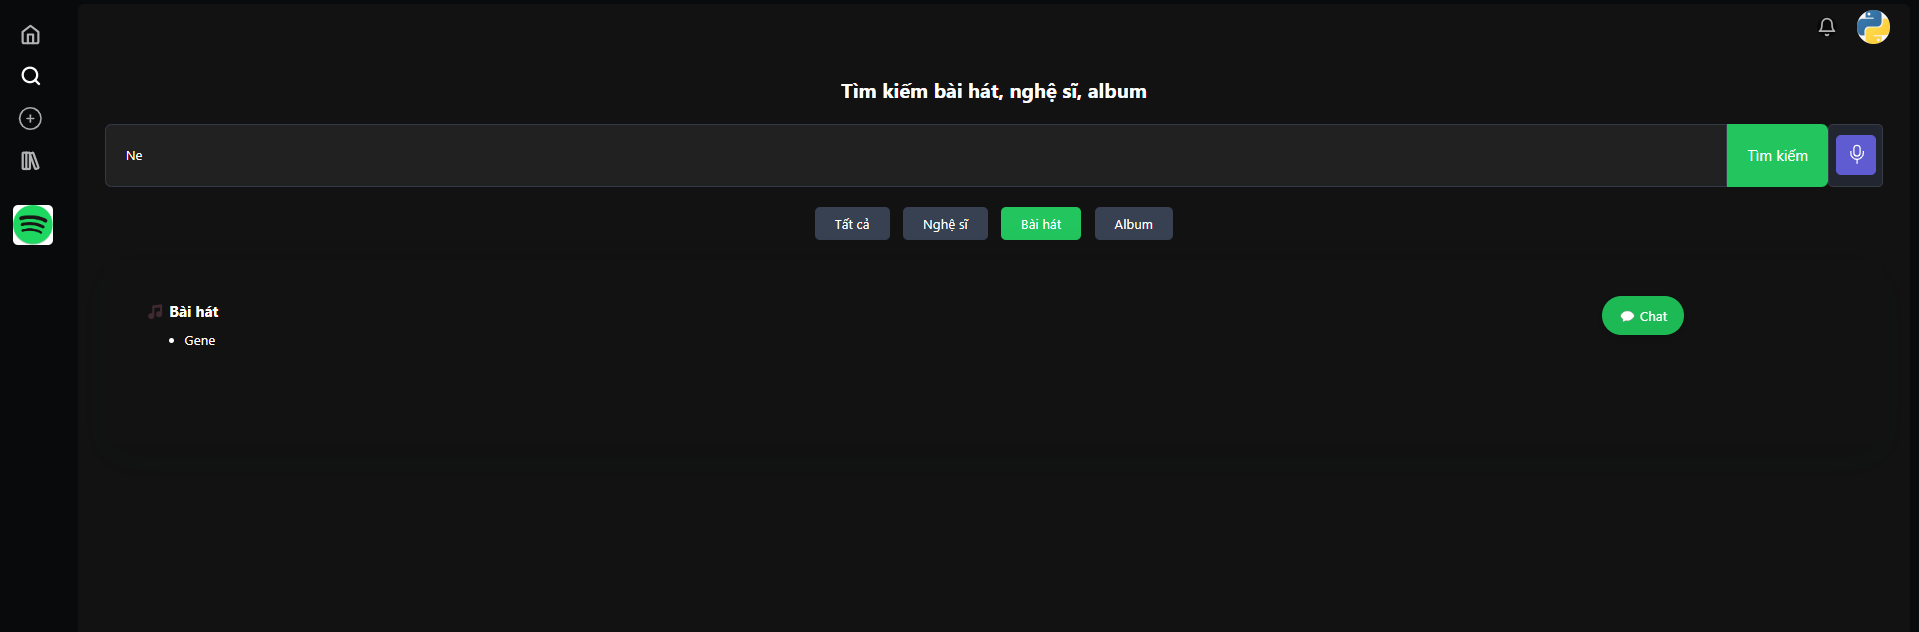
\includegraphics[width=1\textwidth]{imgs/chap5/tim_kiem_3.png}
    \caption{Giao diện tìm kiếm bài hát}
\end{figure}

\begin{figure}[H]
    \centering
    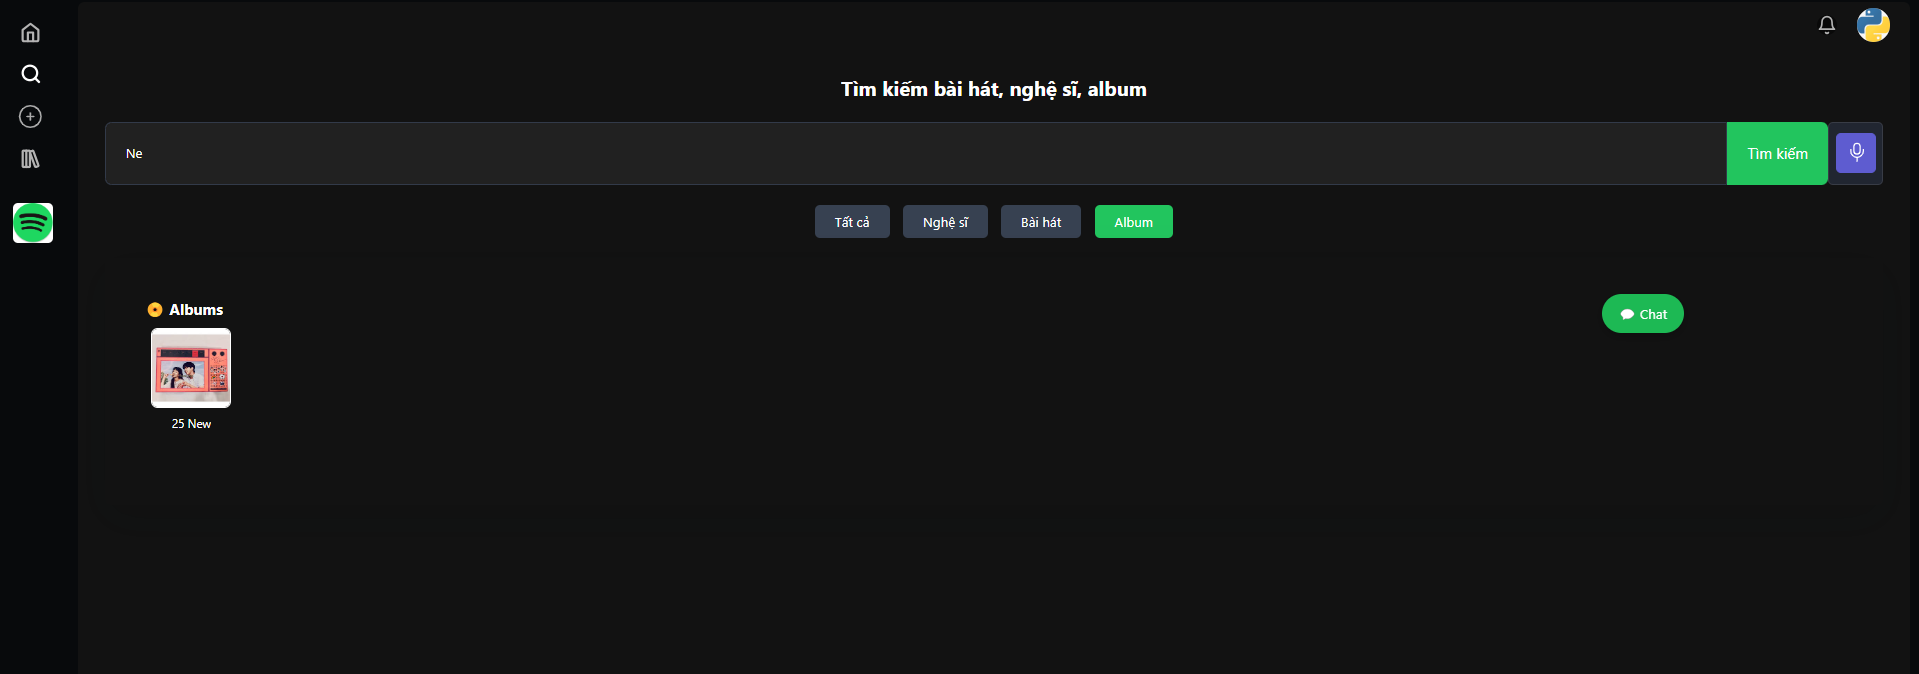
\includegraphics[width=1\textwidth]{imgs/chap5/tim_kiem_4.png}
    \caption{Giao diện tìm kiếm bài hát}
\end{figure}

\subsection{Tìm kiếm bài hát dựa trên tệp ghi âm}
Người dùng có thể ghi âm đoạn bài hát. Hệ thống sử dụng mô hình mã nguồn mở Shazamio để phân tích và trả về dữ liệu của bài hát giống nhất.

\begin{figure}[H]
    \centering
    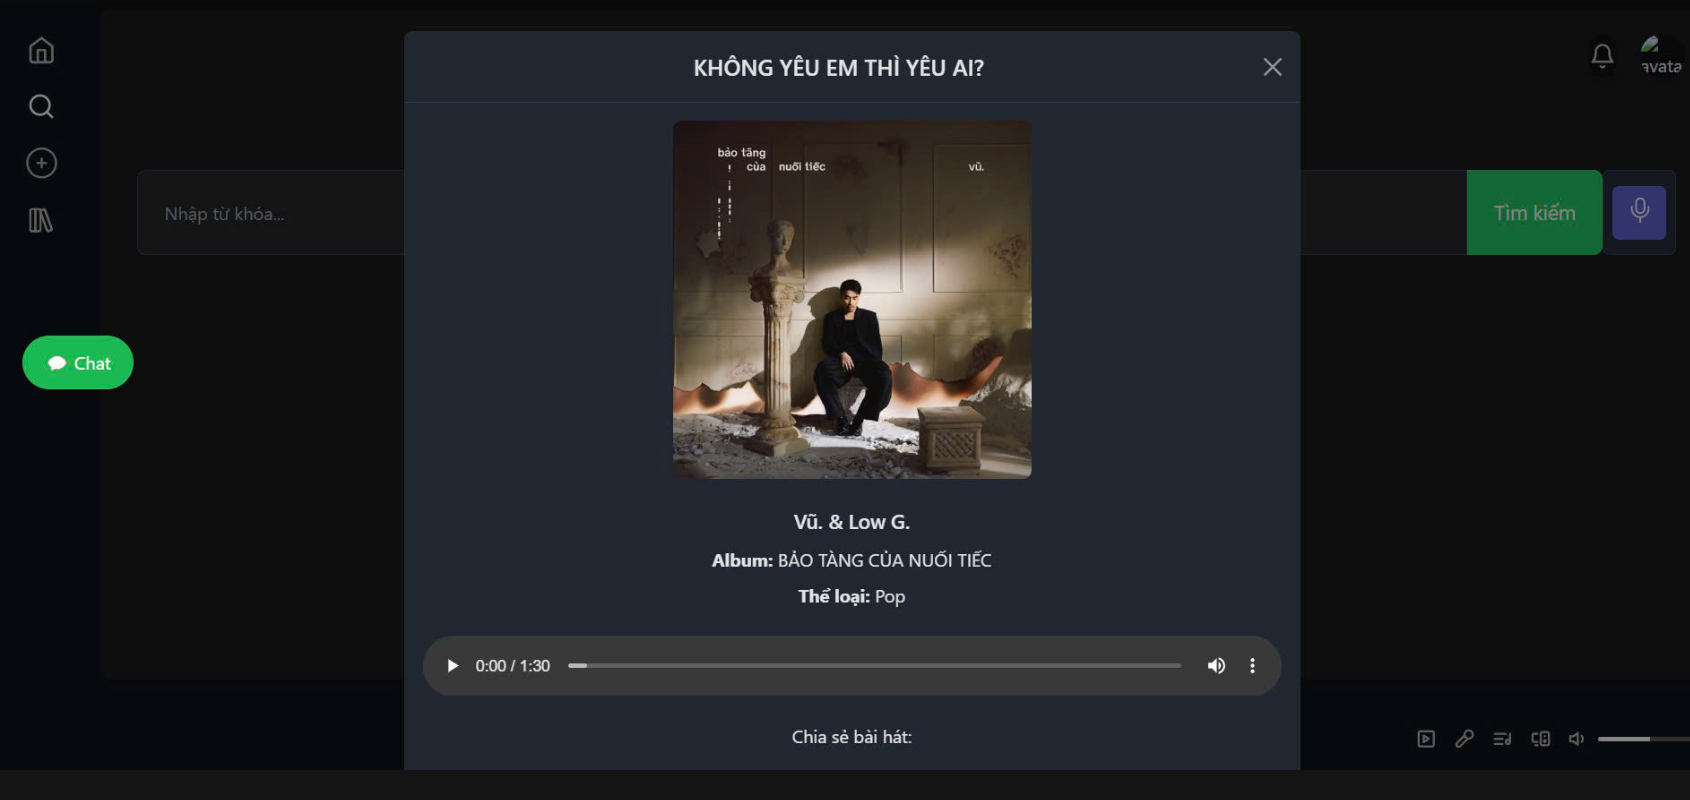
\includegraphics[width=1\textwidth]{imgs/chap5/tim_kiem_5.png}
    \caption{Giao diện tìm kiếm bài hát dựa trên tệp ghi âm}
\end{figure}